\documentclass[10pt,letterpaper]{article}

% ---------------------------------------------------------------------
% Paquetes
% ---------------------------------------------------------------------
\usepackage[utf8]{inputenc}
\usepackage[T1]{fontenc}
\usepackage[spanish,es-noshorthands,es-tabla]{babel}
\usepackage{mathptmx}
\renewcommand{\ttdefault}{lmtt}
\usepackage[margin=0.85in,top=0.9in,bottom=0.9in]{geometry}
\usepackage{fancyhdr}
\usepackage{lastpage}
\usepackage{graphicx}
\usepackage{booktabs}
\usepackage{tabularx}
\usepackage{array}
\usepackage{multirow}
\usepackage{enumitem}
\usepackage{xcolor}
\usepackage{listings}
\usepackage{caption}
\usepackage{titlesec}
\usepackage{natbib}
\usepackage{microtype}
\usepackage[hidelinks]{hyperref}
\usepackage{xurl}
\setlength{\emergencystretch}{3em}
\let\oldUS\_
\renewcommand{\_}{\oldUS\allowbreak}

\setlength{\columnsep}{0.28in}
\setlength{\parindent}{0pt}
\setlength{\parskip}{4pt}
\renewcommand{\arraystretch}{1.15}
\setlist{itemsep=1pt,topsep=3pt,leftmargin=*}
\captionsetup{font=small,labelfont=bf,justification=raggedright,singlelinecheck=false}
\newcolumntype{Y}{>{\raggedright\arraybackslash}X}

\titleformat{\section}{\large\bfseries}{\thesection.}{1.2em}{}
\titleformat{\subsection}{\normalsize\bfseries}{\thesubsection}{1em}{}
\titleformat{\subsubsection}{\normalsize\itshape}{\thesubsubsection}{1em}{}
\titlespacing*{\section}{0pt}{10pt}{5pt}
\titlespacing*{\subsection}{0pt}{8pt}{3pt}

\pagestyle{fancy}
\fancyhf{}
\fancyhead[L]{\small Bases de Datos}
\fancyhead[R]{\small Periodo 2026-2, Proyecto Final, páginas \thepage-\pageref{LastPage}}
\fancyfoot[R]{\small\thepage}
\renewcommand{\headrulewidth}{0pt}
\fancypagestyle{plain}{\fancyhf{}\fancyhead[L]{\small Bases de Datos}\fancyhead[R]{\small Periodo 2026-2, Proyecto Final, páginas \thepage-\pageref{LastPage}}\fancyfoot[R]{\small\thepage}}

\definecolor{codebg}{RGB}{247,247,244}
\definecolor{kw}{RGB}{20,60,120}
\definecolor{cm}{RGB}{110,110,110}
\lstset{
  language=SQL, basicstyle=\ttfamily\scriptsize, keywordstyle=\color{kw}\bfseries,
  commentstyle=\color{cm}\itshape, backgroundcolor=\color{codebg}, frame=none,
  breaklines=true, columns=fullflexible, xleftmargin=4pt, xrightmargin=4pt,
  aboveskip=6pt, belowskip=6pt, showstringspaces=false,
  literate={á}{{\'a}}1 {é}{{\'e}}1 {í}{{\'i}}1 {ó}{{\'o}}1 {ú}{{\'u}}1 {ñ}{{\~n}}1
}

\begin{document}

% ---------------------------------------------------------------------
% Titulo, resumen y abstract (una columna)
% ---------------------------------------------------------------------
\twocolumn[{%
\begin{center}
{\LARGE\bfseries Diseño e implementación de una base de datos para la gestión de portafolios de inversión en una firma de asesoría financiera\par}
\vspace{6pt}
{\large\bfseries Design and implementation of a database for investment portfolio management in a financial advisory firm\par}
\vspace{6pt}
{\bfseries Julian David Rodriguez Ramirez\textsuperscript{1,*} y Juan Esteban Acosta Morales\textsuperscript{1}}\par
\vspace{3pt}
{\small\itshape \textsuperscript{1} Departamento de Matemáticas, Ciencia de Datos, Universidad Externado de Colombia, Bogotá D. C., Colombia}\par
{\small\itshape \textsuperscript{*} julian.rodriguez13@est.uexternado.edu.co, juan.acosta9@est.uexternado.edu.co}\par
\vspace{3pt}
{\small\itshape Docente de Bases de Datos: Martha Liliana Quevedo}\par
\vspace{2pt}
{\small\itshape Proyecto final de Bases de Datos: sistema de gestión de portafolios de inversión}\par
\vspace{8pt}
{\small\bfseries RESUMEN}
\end{center}
\vspace{-4pt}
{\small
Las firmas independientes de asesoría financiera en Colombia suelen gestionar la información de sus clientes, portafolios y comisiones en hojas de cálculo separadas por asesor, lo que impide tener una fuente única y confiable del estado de cada portafolio. Bajo este marco, se diseña e implementa una base de datos relacional en PostgreSQL, complementada con un componente documental en MongoDB, que centraliza clientes, asesores, cuentas, activos (acciones, fondos indexados, CDT y TES), transacciones y rendimientos. El modelo conceptual consta de diez entidades e incluye una especialización disjunta y total de los activos y una entidad débil para los precios históricos; su transformación produce catorce relaciones en forma normal de Boyce-Codd. Dieciséis reglas de negocio se garantizan dentro del propio motor mediante restricciones y disparadores, y la carga de 1.479 transacciones sintéticas sobre precios reales de Yahoo Finance y la TRM oficial no produjo ningún rechazo ni descuadre de saldos. Un portafolio de quince consultas responde las nueve preguntas de información planteadas. Las pruebas con \texttt{EXPLAIN ANALYZE} justificaron dos índices, que redujeron el tiempo de las consultas evaluadas en 49 y 3 veces, y descartaron un tercero por su baja selectividad. Por último, se evidencia una anomalía de actualización perdida entre dos sesiones concurrentes y su corrección mediante bloqueo de fila bajo el nivel de aislamiento \textit{READ COMMITTED}.
\par\vspace{4pt}
\textbf{\textit{Palabras clave:}} bases de datos relacionales; PostgreSQL; modelo entidad-relación extendido; normalización; disparadores; optimización de consultas; control de concurrencia; MongoDB; portafolios de inversión.
\par\vspace{2pt}
\textit{Entrega: 17 de noviembre de 2026.}
}
\begin{center}{\small\bfseries ABSTRACT}\end{center}
\vspace{-4pt}
{\small
Independent financial advisory firms in Colombia often manage client, portfolio and commission data in separate spreadsheets per advisor, which prevents a single reliable source for the state of each portfolio. Within this framework, a relational database is designed and implemented in PostgreSQL, complemented by a document component in MongoDB, that centralizes clients, advisors, accounts, assets (stocks, index funds, certificates of deposit and Colombian treasury bonds), transactions and returns. The conceptual model has ten entities, including a disjoint and total specialization of assets and a weak entity for historical prices; its transformation yields fourteen relations in Boyce-Codd normal form. Sixteen business rules are enforced inside the engine through constraints and triggers, and loading 1,479 synthetic transactions over real Yahoo Finance prices and the official exchange rate produced no rejections or balance mismatches. A set of fifteen queries answers the nine information questions. Tests with \texttt{EXPLAIN ANALYZE} justified two indexes, which reduced the time of the evaluated queries by 49 and 3 times, and ruled out a third one due to its low selectivity. Finally, a lost update anomaly between two concurrent sessions is shown, together with its correction through row locking under the \textit{READ COMMITTED} isolation level.
\par\vspace{4pt}
\textbf{\textit{Keywords:}} relational databases; PostgreSQL; enhanced entity-relationship model; normalization; triggers; query optimization; concurrency control; MongoDB; investment portfolios.
}
\vspace{10pt}
}]

% =====================================================================
\section{Introducción}
% =====================================================================

La firma objeto de este proyecto es una entidad independiente de asesoría financiera en Colombia que gestiona portafolios de inversión para personas naturales. Cada asesor es responsable de un grupo de clientes y ajusta sus portafolios según el perfil de riesgo de cada uno, invirtiendo en acciones, fondos indexados, certificados de depósito a término (CDT) y bonos del Tesoro de Colombia (TES); la firma cobra una comisión fija por cada transacción ejecutada.

Actualmente, la información de clientes, transacciones y portafolios se registra en hojas de cálculo independientes por asesor, complementadas con correos electrónicos para confirmar operaciones. Esta forma de trabajo genera dificultades concretas: no existe una fuente única del estado de cada portafolio, la rentabilidad se calcula de forma manual y propensa a errores, no hay alertas sobre los vencimientos de CDT y TES, no es posible verificar con rapidez si la diversificación de un portafolio respeta el perfil de riesgo del cliente, y consolidar lo facturado en comisiones por asesor o por periodo exige un trabajo manual considerable. Como señalan \citet{elmasri2016} y \citet{silberschatz2019}, la dispersión de los datos en archivos independientes, frente al modelo relacional propuesto por \citet{codd1970}, conduce a redundancia, inconsistencias y dificultades de acceso que un sistema de bases de datos busca resolver.

Bajo este marco, se plantea la pregunta que guía el proyecto: \textbf{¿cómo debe estructurarse una base de datos que garantice la consistencia de la información de los portafolios y permita responder las preguntas de negocio de la firma?}

\subsection{Objetivos}

\subsubsection{Objetivo general}

Diseñar, implementar, evaluar y documentar una base de datos que centralice la información de clientes, asesores, activos, transacciones y comisiones, de modo que permita calcular de forma confiable la rentabilidad y la diversificación de cada portafolio, generar alertas de vencimiento de los instrumentos de renta fija y consolidar el análisis de comisiones.

\subsubsection{Objetivos específicos}

\begin{itemize}
  \item Construir un modelo conceptual entidad-relación extendido que represente las reglas de negocio del dominio y transformarlo en un esquema relacional en forma normal de Boyce-Codd.
  \item Garantizar dentro del motor, mediante restricciones y disparadores, las reglas de negocio que no dependen de la aplicación.
  \item Responder las nueve preguntas de información mediante consultas SQL y vistas reutilizables.
  \item Evaluar con planes de ejecución la pertinencia de los índices y demostrar el comportamiento transaccional ante accesos concurrentes.
  \item Identificar una parte del problema adecuada para un modelo documental e implementarla en MongoDB.
\end{itemize}

\subsection{Alcance}

El proyecto incluye la gestión de clientes y su perfil de riesgo; la asignación de clientes a asesores; el registro de los cuatro tipos de activo; los precios históricos de acciones y fondos, obtenidos de Yahoo Finance mediante la librería \texttt{yfinance} \citep{yfinance}, y la Tasa Representativa del Mercado (TRM) publicada por la Superintendencia Financiera \citep{trm}, ambos en carga por lotes; las compras, ventas, depósitos y retiros; los dividendos e intereses; y el cálculo de rentabilidad, diversificación, vencimientos y comisiones. Quedan por fuera el trading en tiempo real, la integración en vivo con bolsas o corredores, el cálculo tributario, la contabilidad interna de la firma y la atención al cliente. Todos los valores del sistema se expresan en dólares; los CDT y TES, que se pactan en pesos, se convierten con la TRM vigente en la fecha de cada operación.

% =====================================================================
\section{Requerimientos y reglas de negocio}
% =====================================================================

Las doce reglas de la formulación se mantuvieron y se precisaron durante el modelado; adicionalmente, se identificaron cuatro reglas nuevas (13 a 16). La Tabla~\ref{tab:reglas} resume cada regla y el mecanismo con el que el motor la garantiza.

\begin{table*}[t]
\centering
\small
\caption{Reglas de negocio y mecanismo con el que se garantizan en PostgreSQL.}
\label{tab:reglas}
\begin{tabularx}{\textwidth}{@{}c Y Y@{}}
\toprule
\textbf{\#} & \textbf{Regla de negocio} & \textbf{Mecanismo en la base de datos} \\
\midrule
1 & Cada cliente tiene un único perfil de riesgo (conservador, moderado o agresivo). & Clave foránea \texttt{cliente.id\_perfil} NOT NULL. \\
2 & El porcentaje en renta variable no debe superar el límite del perfil: 20\,\%, 50\,\% o 100\,\%. & Atributo del perfil y vista de control \texttt{v\_cumplimiento\_perfil}. \\
3 & Cada cliente está asignado a un único asesor; un asesor gestiona varios clientes. & Clave foránea \texttt{cliente.id\_asesor} NOT NULL. \\
4 & Toda compra requiere saldo suficiente para el monto más la comisión. & Disparador \texttt{trg\_transaccion\_validar} y CHECK \texttt{saldo\_efectivo >= 0}. \\
5 & Toda compra o venta genera una comisión del 0,5\,\% de su valor. & \texttt{tasa\_comision} con valor por defecto 0,005 y columna generada \texttt{comision}. \\
6 & Los CDT y TES no se venden antes de su vencimiento y se redimen por el total. & Disparador \texttt{trg\_transaccion\_validar}. \\
7 & La tasa de un CDT o TES se pacta en la compra y no cambia. & Atributo \texttt{transaccion.tasa\_pactada}, obligatorio en esas compras. \\
8 & Los dividendos e intereses son ingresos de la cuenta. & Tabla \texttt{rendimiento} y disparador \texttt{trg\_rendimiento\_aplicar}. \\
9 & Las acciones y fondos se valoran con el precio más reciente disponible. & Tabla \texttt{precio\_historico} y función \texttt{fn\_precio}. \\
10 & Un cliente puede tener varias cuentas; cada cuenta pertenece a un único cliente. & Clave foránea \texttt{cuenta.id\_cliente} NOT NULL. \\
11 & No se vende una cantidad mayor a la que se posee. & Función \texttt{fn\_tenencia} y disparador de transacción. \\
12 & Cada activo es de un único tipo, que determina sus atributos. & Especialización disjunta (clave foránea compuesta y CHECK) y total (disparador diferido). \\
13 & El sistema valora en USD; los CDT y TES se convierten con la TRM vigente. & Tabla \texttt{trm} y función \texttt{fn\_trm}. \\
14 & El efectivo solo cambia por operaciones registradas. & Disparador \texttt{trg\_cuenta\_proteger\_saldo}. \\
15 & Transacciones, movimientos y rendimientos no se modifican ni se eliminan. & Disparadores \texttt{trg\_*\_inmutable}. \\
16 & Solo se vinculan mayores de edad; documento y correo no se repiten. & CHECK de edad y restricciones UNIQUE. \\
\bottomrule
\end{tabularx}
\end{table*}

La base de datos debe responder las siguientes preguntas de información, que guían el diseño de las consultas de la Sección~\ref{sec:consultas}:

\begin{enumerate}[label=P\arabic*.]
  \item ¿Cuál es el valor actual del portafolio de cada cliente, desglosado por tipo de activo?
  \item ¿Cuál es la rentabilidad de cada cliente en los últimos 12 meses?
  \item ¿Qué porcentaje del portafolio está en cada tipo de activo y se cumple el límite del perfil?
  \item ¿Qué CDT y TES vencen en los próximos 30, 60 y 90 días, y a qué clientes pertenecen?
  \item ¿Cuánto ha generado cada asesor en comisiones durante un periodo?
  \item ¿Qué clientes tienen la mayor y la menor rentabilidad?
  \item ¿Cuál es el historial completo de transacciones de un cliente?
  \item ¿Cuántos clientes gestiona cada asesor y cuál es el valor que administra (AUM)?
  \item ¿Cuáles son los activos más comprados y más vendidos en un periodo?
\end{enumerate}

% =====================================================================
\section{Modelo conceptual}
% =====================================================================

El modelo conceptual, presentado en la Figura~\ref{fig:eer} con la notación entidad-relación extendida de \citet{elmasri2016}, consta de diez entidades: Asesor, PerfilRiesgo, Cliente, Cuenta, MovimientoEfectivo, Activo, Transacción, Rendimiento, PrecioHistórico y TRM.

\begin{figure*}[t]
\centering
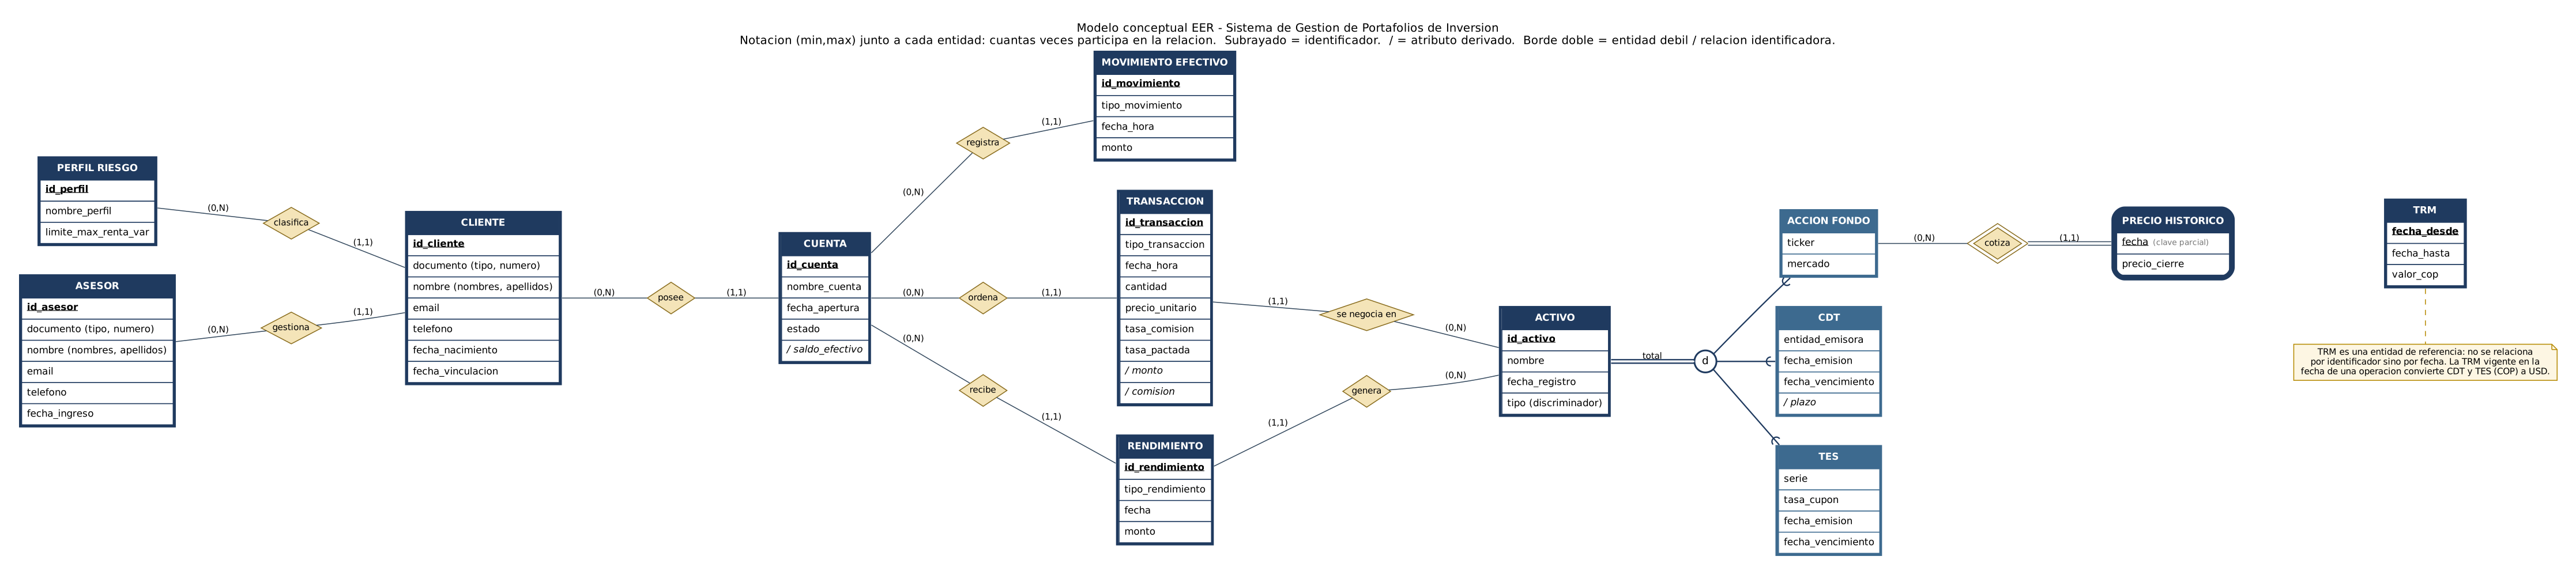
\includegraphics[width=\textwidth]{eer_conceptual.png}
\caption{Modelo conceptual entidad-relación extendido. Los pares (mín, máx) junto a cada entidad indican cuántas veces participa en la relación; el subrayado señala identificadores y la barra, atributos derivados.}
\label{fig:eer}
\end{figure*}

\textbf{Cardinalidades.} Todas las relaciones son de uno a muchos. El lado N participa de forma obligatoria (1,1) y el lado 1 de forma opcional (0,N). Por ejemplo, un cliente tiene exactamente un perfil y un asesor, mientras que un perfil o un asesor recién creado puede no tener clientes. Del mismo modo, cada movimiento, transacción o rendimiento pertenece a una sola cuenta, y una cuenta recién abierta no tiene ninguno.

\textbf{Especialización de Activo.} La especialización en AcciónFondo, CDT y TES es necesaria porque los subtipos tienen atributos distintos (ticker y mercado; entidad emisora y fechas; serie y cupón) y porque solo AcciónFondo tiene precios de mercado. Es \textit{disjunta}, porque un instrumento no puede ser a la vez CDT y TES, y \textit{total}, porque no existe un activo sin tipo. Acción y fondo forman un solo subtipo, ya que comparten atributos y relaciones y el discriminador los distingue.

\textbf{Entidad débil.} PrecioHistórico depende existencialmente de AcciónFondo y se identifica con la clave de su propietario más la fecha, que actúa como clave parcial.

\textbf{Transacción como entidad.} No se modela como una relación muchos a muchos entre Cuenta y Activo porque la misma cuenta compra el mismo activo muchas veces, y cada ocurrencia tiene atributos propios (fecha, cantidad, precio y tasa).

No se usaron categorías ni agregación, ya que ninguna regla del dominio las requiere; tampoco se generalizaron Asesor y Cliente en una entidad Persona, pues no comparten relaciones.

% =====================================================================
\section{Modelo relacional y normalización}
% =====================================================================

\subsection{Transformación al modelo relacional}

Las diez entidades se transforman en catorce relaciones (Figura~\ref{fig:relacional}). Cada entidad fuerte origina una tabla con clave sustituta, mientras que los documentos de identidad y los correos se conservan como claves candidatas mediante restricciones UNIQUE. Las relaciones de uno a muchos se resuelven con la clave foránea en el lado N. La especialización se transforma en una tabla para el supertipo y una por subtipo, que comparten la clave primaria; cada subtipo repite además \texttt{id\_tipo\_activo} para referenciar al supertipo con una clave foránea compuesta, lo que garantiza que la especialización sea disjunta. La entidad débil toma la clave primaria compuesta \texttt{(id\_activo, fecha)}.

\begin{figure*}[p]
\centering
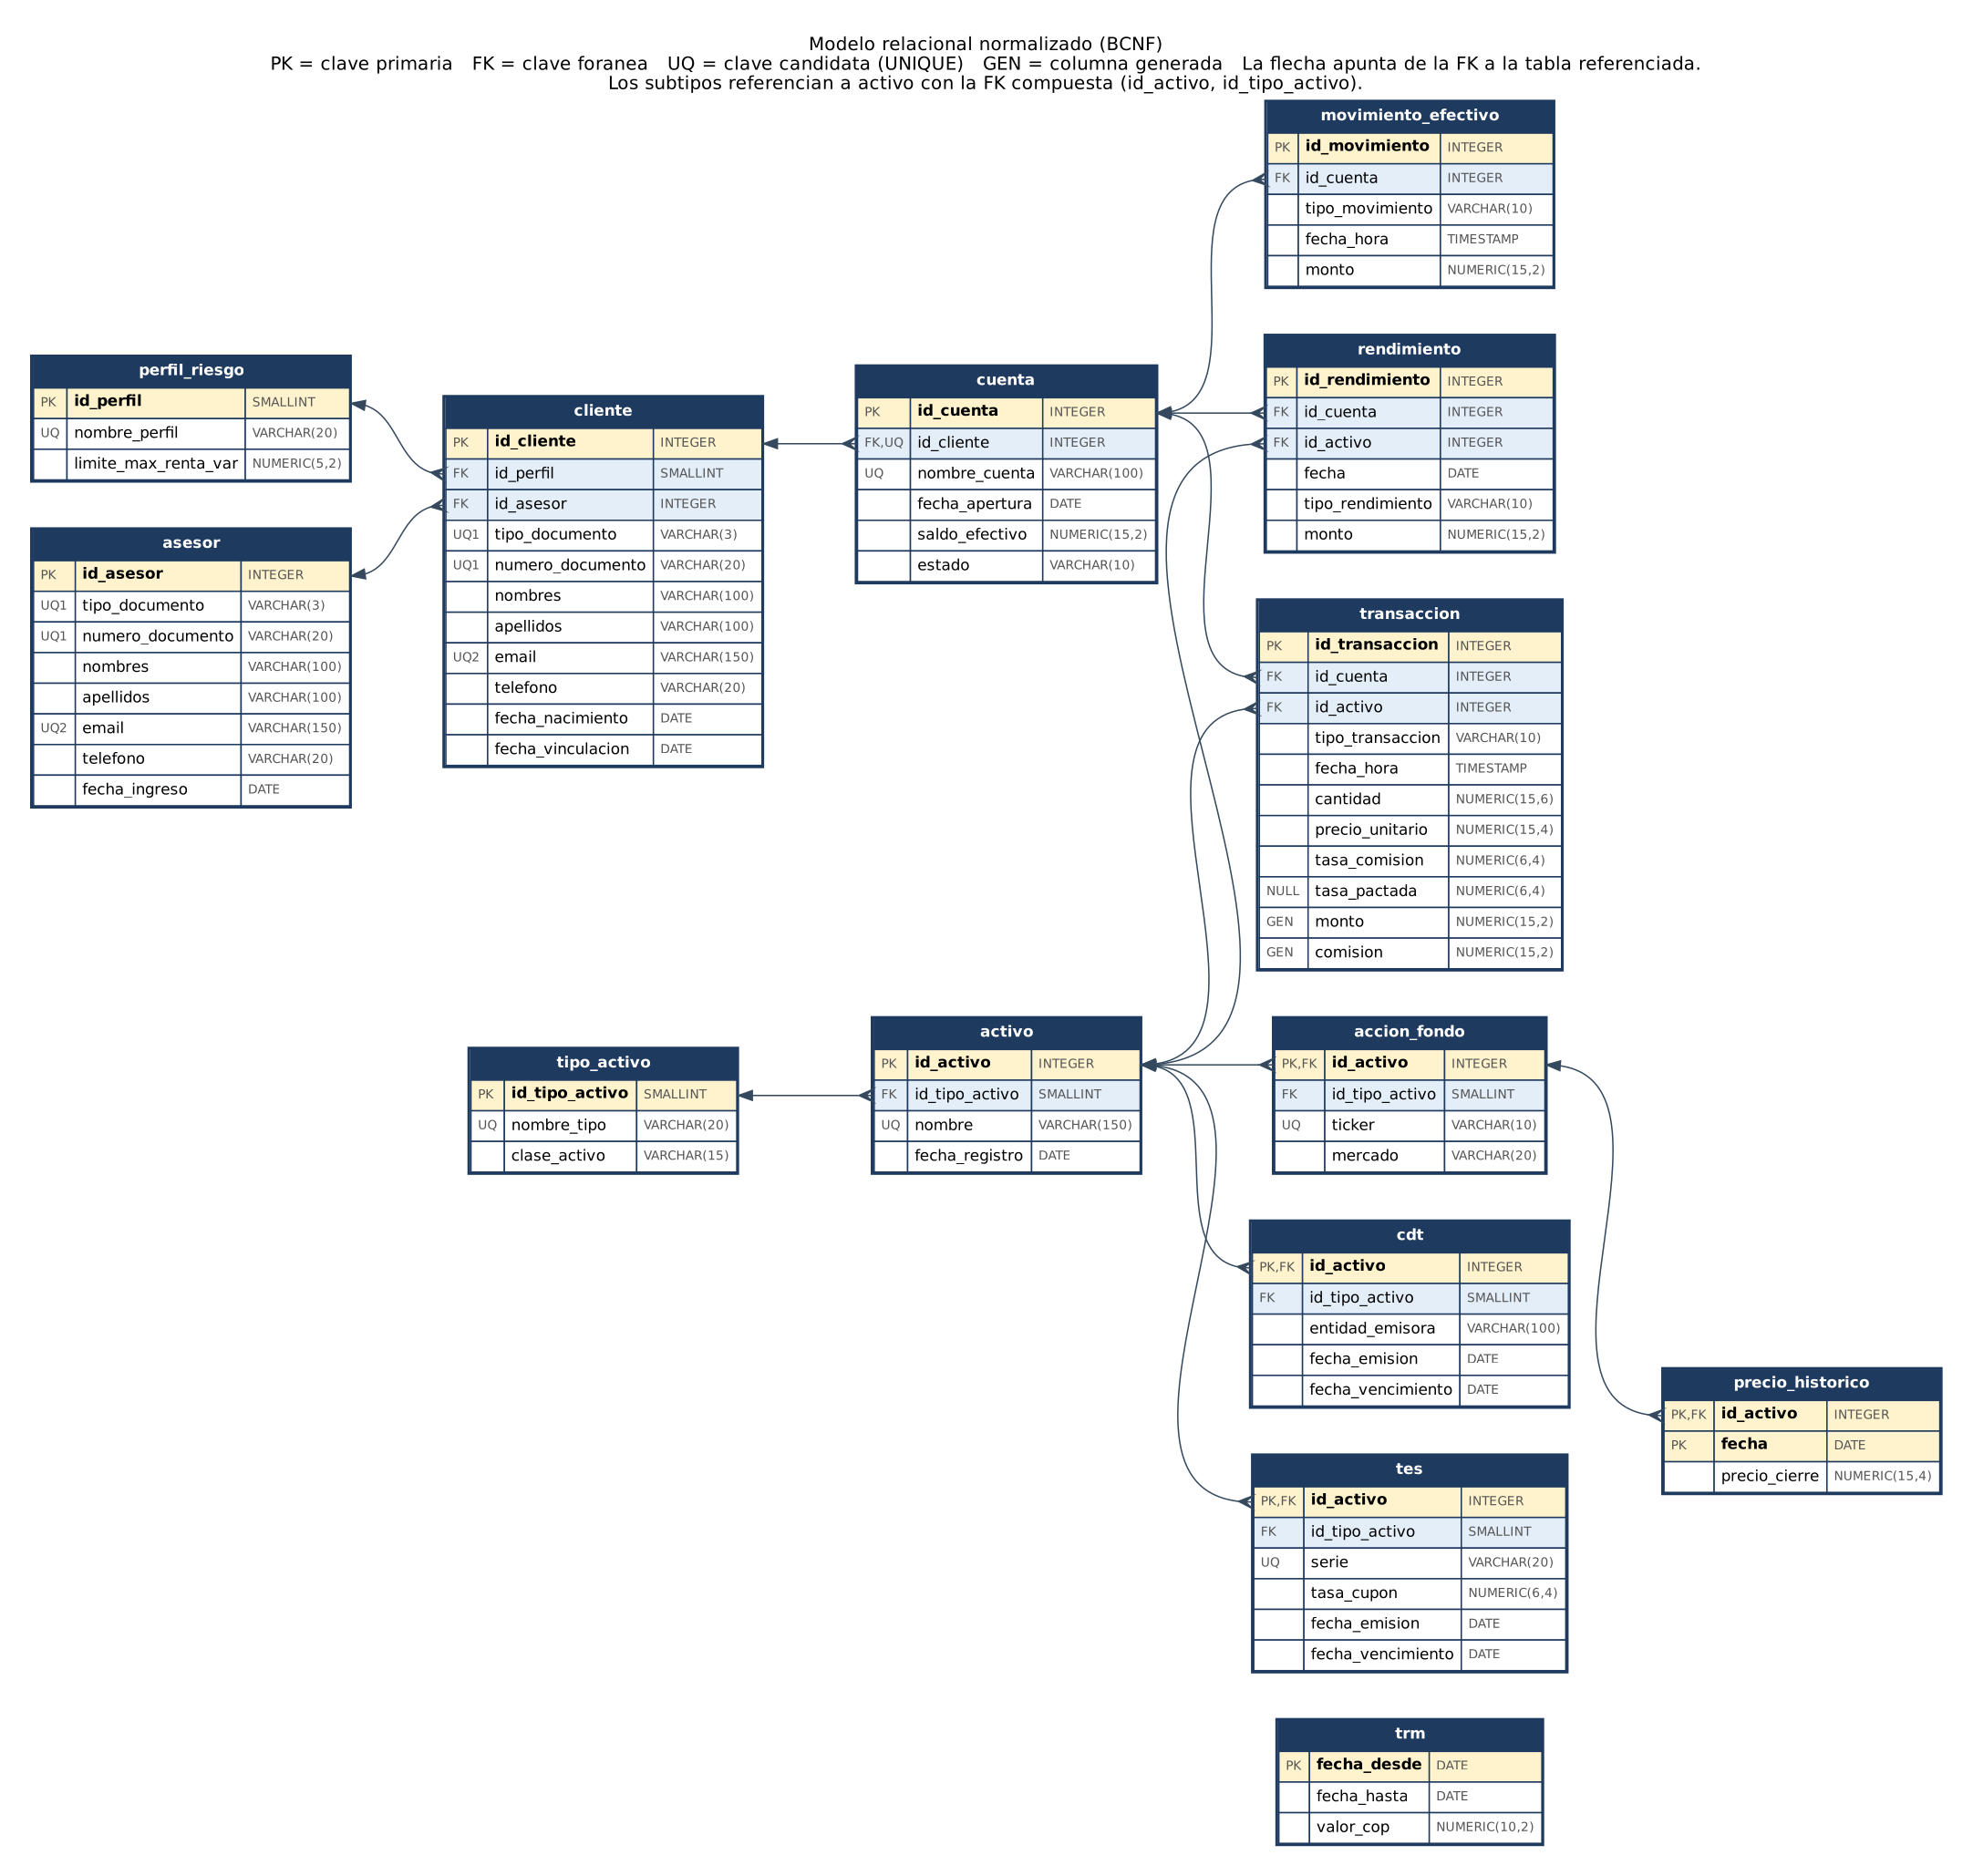
\includegraphics[width=0.93\textwidth]{modelo_relacional.png}
\caption{Modelo relacional normalizado. PK: clave primaria; FK: clave foránea; UQ: clave candidata; GEN: columna generada. Las flechas van de la clave foránea a la tabla referenciada.}
\label{fig:relacional}
\end{figure*}

\subsection{Dependencias funcionales y formas normales}

Se partió del modelo relacional preliminar y se verificó cada forma normal:

\begin{itemize}
  \item \textbf{1FN.} Todos los atributos son atómicos: el documento y el nombre se separaron en sus componentes, y los precios, que en el modelo conceptual son un atributo multivaluado, se llevaron a su propia tabla.
  \item \textbf{2FN.} La única clave compuesta es \texttt{(id\_activo, fecha)} y el atributo \texttt{precio\_cierre} depende de ambas partes. Se eliminó el atributo \texttt{fuente}, que era constante.
  \item \textbf{3FN.} Se eliminaron cinco dependencias transitivas del diseño preliminar: \texttt{monto} dependía de cantidad $\times$ precio y \texttt{comision} de monto $\times$ tarifa, por lo que ambas pasaron a ser columnas generadas; \texttt{plazo\_categoria} dependía del vencimiento del TES y se eliminó; \texttt{tasa\_fija} y \texttt{monto\_principal} describían la compra y no el CDT, por lo que pasaron a la transacción; y \texttt{moneda} dependía del tipo de activo y se eliminó al valorar todo en dólares.
  \item \textbf{FNBC.} En cada relación, el determinante de toda dependencia funcional no trivial es una clave candidata. Por ejemplo, en \texttt{cliente} los determinantes son el identificador, el documento y el correo, y los tres son claves candidatas. Ninguna relación requirió descomposición adicional.
\end{itemize}

\subsection{Redundancias controladas}

El saldo de efectivo de la cuenta puede derivarse del historial de operaciones; sin embargo, se almacena para validar cada compra bloqueando una sola fila. Esta redundancia controlada no viola ninguna forma normal, porque depende de filas de otras tablas y no de otro atributo de la misma relación, y se protege con tres mecanismos: solo los disparadores pueden modificarla, el historial es inmutable y una consulta de auditoría verifica que el saldo almacenado coincida con el reconstruido.

% =====================================================================
\section{Diccionario de datos}
% =====================================================================

El diccionario completo, con las 78 columnas de las catorce tablas, se encuentra en el repositorio del proyecto. La Tabla~\ref{tab:diccionario} resume las columnas que concentran las reglas de negocio.

\begin{table*}[t]
\centering
\small
\caption{Columnas del diccionario de datos que concentran las reglas de negocio.}
\label{tab:diccionario}
\begin{tabularx}{\textwidth}{@{}l l l Y@{}}
\toprule
\textbf{Tabla.columna} & \textbf{Tipo} & \textbf{Restricción} & \textbf{Descripción} \\
\midrule
perfil\_riesgo.limite\_max\_renta\_var & NUMERIC(5,2) & CHECK entre 0 y 100 & Porcentaje máximo en acciones y fondos (Regla 2) \\
cliente.fecha\_vinculacion & DATE & CHECK de mayoría de edad & Solo personas mayores de edad (Regla 16) \\
cuenta.saldo\_efectivo & NUMERIC(15,2) & CHECK $\geq$ 0 & Efectivo en USD; redundancia controlada \\
activo.id\_tipo\_activo & SMALLINT & FK, discriminador & 1 acción, 2 fondo, 3 CDT, 4 TES (Regla 12) \\
precio\_historico.precio\_cierre & NUMERIC(15,4) & CHECK $>$ 0; PK (id\_activo, fecha) & Precio de cierre diario en USD (Regla 9) \\
trm.valor\_cop & NUMERIC(10,2) & CHECK $>$ 0 & Pesos por dólar en su rango de vigencia \\
transaccion.cantidad & NUMERIC(15,6) & CHECK $>$ 0 & Unidades o títulos negociados \\
transaccion.tasa\_comision & NUMERIC(6,4) & DEFAULT 0,005 & Tarifa vigente en la operación (Regla 5) \\
transaccion.tasa\_pactada & NUMERIC(6,4) & Solo en CDT y TES & Tasa efectiva anual pactada (Regla 7) \\
transaccion.monto & NUMERIC(15,2) & Columna generada & cantidad $\times$ precio\_unitario \\
transaccion.comision & NUMERIC(15,2) & Columna generada & monto $\times$ tasa\_comision \\
\bottomrule
\end{tabularx}
\end{table*}

% =====================================================================
\section{Implementación en PostgreSQL}
% =====================================================================

La base de datos se construye desde cero con un único comando (\texttt{EJECUTAR\_TODO.bat}), que ejecuta los scripts en orden y guarda la salida de cada paso como evidencia; se probó en PostgreSQL 16 y 18 \citep{postgresql}. La Tabla~\ref{tab:scripts} describe los scripts.

\begin{table}[h]
\centering
\small
\caption{Scripts de la implementación.}
\label{tab:scripts}
\begin{tabularx}{\columnwidth}{@{}l Y@{}}
\toprule
\textbf{Script} & \textbf{Contenido} \\
\midrule
01\_ddl & 14 tablas con PK, FK, UNIQUE, CHECK, DEFAULT y columnas generadas \\
02\_funciones\_triggers & 7 funciones, 6 disparadores y el procedimiento \texttt{sp\_registrar\_compra} \\
03\_carga\_catalogos & Perfiles de riesgo y tipos de activo \\
04\_carga\_datos & Datos generados por \texttt{generar\_datos.py} \\
05\_vistas & 5 vistas reutilizables \\
06\_consultas & 15 consultas \\
07\_optimizacion & Pruebas con EXPLAIN ANALYZE \\
08\_transacciones & Pruebas de propiedades ACID \\
\bottomrule
\end{tabularx}
\end{table}

\subsection{Disparadores}

Las reglas que comparan datos de varias tablas no pueden expresarse con una restricción CHECK, por lo que se implementaron con disparadores. El principal, \texttt{trg\_transaccion\_validar}, se ejecuta antes de cada inserción en \texttt{transaccion}: bloquea la fila de la cuenta, obtiene el tipo y el vencimiento del activo, calcula el monto y la comisión, valida las reglas 4, 6, 7 y 11 según se trate de una compra o una venta, y actualiza el saldo. El siguiente fragmento muestra la validación del saldo:

\begin{lstlisting}
SELECT saldo_efectivo INTO v_saldo
FROM cuenta WHERE id_cuenta = NEW.id_cuenta
FOR UPDATE;
...
IF v_saldo < v_monto + v_comision THEN
  RAISE EXCEPTION 'Regla 4: saldo insuficiente';
END IF;
UPDATE cuenta
SET saldo_efectivo = saldo_efectivo - (v_monto + v_comision)
WHERE id_cuenta = NEW.id_cuenta;
\end{lstlisting}

Los demás disparadores aplican depósitos, retiros y rendimientos al saldo; impiden modificar el saldo directamente; impiden editar o eliminar el historial; y exigen, al confirmar la transacción, que todo activo tenga su fila de subtipo.

\subsection{Carga de datos}

Los precios de cierre diarios y los dividendos de diez acciones y fondos se descargaron de Yahoo Finance desde enero de 2024, y la TRM oficial desde el portal de datos abiertos del Estado colombiano \citep{trm}. Asesores, clientes y operaciones son sintéticos y se generan con una semilla fija para que la carga sea reproducible. Cada operación pasa por los disparadores, de modo que todos los datos cumplen las reglas de negocio. La Tabla~\ref{tab:registros} muestra el volumen cargado.

\begin{table}[h]
\centering
\small
\caption{Registros cargados por tabla.}
\label{tab:registros}
\begin{tabular}{@{}l r@{}}
\toprule
\textbf{Tabla} & \textbf{Registros} \\
\midrule
precio\_historico & 7.220 \\
transaccion & 1.479 \\
rendimiento & 1.367 \\
trm & 698 \\
movimiento\_efectivo & 407 \\
activo (333 CDT, 3 TES, 10 acciones y fondos) & 346 \\
cuenta & 80 \\
cliente & 60 \\
asesor & 6 \\
\bottomrule
\end{tabular}
\end{table}

La carga no produjo ningún rechazo de los disparadores. Adicionalmente, se verificó que la base rechaza dieciséis operaciones inválidas, una por regla, entre ellas una compra sin saldo, una venta sin tenencia, la venta de un CDT antes de su vencimiento, la modificación directa del saldo y la vinculación de un menor de edad.

% =====================================================================
\section{Consultas SQL y resultados}\label{sec:consultas}
% =====================================================================

Cada pregunta de información tiene al menos una consulta que la responde. Las consultas utilizan combinaciones de varias tablas, agrupaciones con GROUP BY y HAVING, expresiones CASE, subconsultas, expresiones de tabla comunes (WITH) y funciones de ventana. La Tabla~\ref{tab:consultas} resume las consultas y su resultado con los datos cargados al 17 de noviembre de 2026.

\begin{table*}[t]
\centering
\small
\caption{Consultas, pregunta que responden, técnicas utilizadas y resultado.}
\label{tab:consultas}
\begin{tabularx}{\textwidth}{@{}l l l Y@{}}
\toprule
\textbf{Consulta} & \textbf{Pregunta} & \textbf{Técnicas} & \textbf{Resultado} \\
\midrule
C01 & P1 & Vista, SUM con CASE & 60 clientes; el mayor portafolio vale 694.877 USD \\
C02 & P2 & Función de rentabilidad & Rentabilidades entre 1,60\,\% y 34,67\,\% \\
C03 & P3 & Vistas, subconsulta en FROM, CASE & 11 de 60 clientes exceden su límite (6 moderados y 5 conservadores) \\
C04 & P4 & Vista, CASE & 44 CDT vencen en 90 días (16, 14 y 14 por ventana) \\
C05 & P5 & JOIN de cuatro tablas, GROUP BY & 23.199 USD en comisiones en los últimos 12 meses \\
C06 & P6 & WITH, RANK & Mayor rentabilidad 34,67\,\%; menor 1,60\,\% \\
C07 & P7 & JOIN, suma acumulada con OVER & Historial con flujo de caja acumulado \\
C08 & P8 & WITH, LEFT JOIN & AUM total de 10,14 millones de USD \\
C09 & P9 & GROUP BY, ORDER BY, LIMIT & Más comprado: Alphabet (165.922 USD); más vendido: Johnson \& Johnson (183.149 USD) \\
C10 & Apoyo P5 & HAVING con subconsulta & 3 asesores superan el promedio de comisiones \\
C11 & Apoyo P2 & WITH, LAG & Variación del precio promedio mensual de 10 activos \\
C12 & Apoyo P1 & WITH y vista & Mayor ganancia no realizada: Bancolombia, 115.787 USD \\
C13 & Apoyo P7 & Subconsulta correlacionada NOT EXISTS & 18 clientes sin operaciones en 90 días \\
C14 & Apoyo P9 & GROUP BY y HAVING & 13 activos presentes en 3 o más cuentas \\
C15 & Integridad & Función de auditoría & 0 cuentas con saldo descuadrado \\
\bottomrule
\end{tabularx}
\end{table*}

Las consultas se apoyan en cinco vistas: \texttt{v\_tenencia}, que calcula lo que cada cuenta posee; \texttt{v\_posicion\_actual}, que valora cada posición; \texttt{v\_portafolio\_cliente}, que agrupa el valor por categoría incluyendo el efectivo; \texttt{v\_cumplimiento\_perfil}, que calcula el porcentaje en renta variable (Regla 2); y \texttt{v\_vencimientos\_renta\_fija} (P4). Como ejemplo, la consulta C03b identifica a los clientes que exceden el límite de su perfil:

\begin{lstlisting}
SELECT cliente, nombre_perfil, limite_pct,
       pct_renta_variable,
       CASE WHEN pct_renta_variable <= limite_pct
            THEN 'CUMPLE' ELSE 'EXCEDE' END AS estado
FROM v_cumplimiento_perfil
ORDER BY estado DESC, pct_renta_variable DESC;
\end{lstlisting}

La valoración de un CDT o TES lleva el monto invertido a pesos con la TRM de la fecha de compra, lo capitaliza a la tasa pactada $i$ durante $d$ días y lo devuelve a dólares con la TRM de la fecha de valoración:
\begin{equation}
V_{USD} = \frac{M_{USD}\cdot TRM_{compra}\cdot(1+i)^{d/365}}{TRM_{hoy}}.
\end{equation}
La rentabilidad de un cliente en un periodo se calcula a partir de los valores inicial $V_i$ y final $V_f$ de sus cuentas y de los aportes netos $F$:
\begin{equation}
r = \frac{V_f - V_i - F}{V_i + F}\times 100.
\end{equation}

% =====================================================================
\section{Optimización y planes de ejecución}
% =====================================================================

Se evaluaron tres hipótesis de mejora con \texttt{EXPLAIN ANALYZE}. Las pruebas se realizaron sobre copias de las tablas en un esquema aparte, para no alterar la base, y sin paralelismo, para que los tiempos fueran comparables. La Tabla~\ref{tab:optimizacion} resume los resultados.

\begin{table*}[t]
\centering
\small
\caption{Pruebas de optimización: tiempo de ejecución y plan antes y después de cada cambio.}
\label{tab:optimizacion}
\begin{tabularx}{\textwidth}{@{}l r r Y l@{}}
\toprule
\textbf{Prueba} & \textbf{Antes} & \textbf{Después} & \textbf{Cambio en el plan} & \textbf{Decisión} \\
\midrule
1. Último precio de cada posición & 103,5 ms & 2,1 ms & Seq Scan y Sort por posición $\rightarrow$ Index Scan Backward con Limit & PK (id\_activo, fecha) \\
2. Historial de un cliente (221.850 filas) & 22,4 ms & 7,7 ms & Seq Scan $\rightarrow$ Bitmap Index Scan por cuenta & Índice (id\_cuenta, fecha\_hora) \\
3. Compras por activo & 40,8 ms & 44,2 ms & Seq Scan en ambos casos & Índice descartado \\
\bottomrule
\end{tabularx}
\end{table*}

\textbf{Prueba 1.} El diseño preliminar tenía \texttt{precio\_historico} con una clave sustituta. La hipótesis fue que buscar el último precio de un activo obliga a recorrer y ordenar las 7.220 filas una vez por cada posición, y que un índice B-tree sobre \texttt{(id\_activo, fecha)} permitiría ir directamente a la fecha más reciente. El tiempo se redujo 49 veces, lo que justifica la clave primaria compuesta del modelo final.

\textbf{Prueba 2.} Con una copia ampliada de las transacciones, que simula el crecimiento de la firma, el filtro por las cuentas de un cliente es muy selectivo (cerca de 1/80 de las filas). El índice compuesto redujo el tiempo cerca de 3 veces y se creó en la base real, donde también lo aprovecha la función \texttt{fn\_tenencia}.

\textbf{Prueba 3.} Se planteó un índice sobre \texttt{tipo\_transaccion}, pero la columna solo tiene dos valores y el 76\,\% de las filas son compras. El planificador mantuvo el recorrido secuencial y el tiempo no mejoró (40,8 frente a 44,2 ms, una variación propia de la medición), por lo que el índice no es pertinente: ocuparía 1,5 MB y haría más lentas las escrituras sin ningún beneficio.

% =====================================================================
\section{Transacciones y concurrencia}
% =====================================================================

La compra es la operación atómica central del sistema: validar el saldo, registrar la transacción con su comisión y descontar el efectivo deben ocurrir juntos o no ocurrir. Las propiedades ACID se evidenciaron de la siguiente manera:

\begin{itemize}
  \item \textbf{Atomicidad:} un depósito seguido de una compra imposible en la misma transacción termina en ROLLBACK, y el depósito también se deshace.
  \item \textbf{Consistencia:} la base rechaza modificar el saldo, eliminar una transacción o retirar más de lo disponible.
  \item \textbf{Aislamiento:} el disparador bloquea la fila de la cuenta con \texttt{SELECT ... FOR UPDATE}.
  \item \textbf{Durabilidad:} los cambios confirmados persisten en el registro de escritura anticipada del motor.
\end{itemize}

\textbf{Escenario de concurrencia.} Dos asesores registran al mismo tiempo una compra sobre la misma cuenta, cuyo saldo alcanza para una sola. Se ejecutaron dos sesiones reales en paralelo (Tabla~\ref{tab:concurrencia}). Sin bloqueo, ambas sesiones leyeron un saldo de 1.000 USD y aprobaron una compra de 700 USD; el saldo final fue de 300 USD con dos compras aprobadas, cuando el valor correcto habría sido $-400$. Esta anomalía corresponde a una actualización perdida \citep{berenson1995}. Con el disparador real, la segunda sesión esperó a que la primera confirmara, volvió a leer el saldo ya descontado y fue rechazada.

\begin{table}[h]
\centering
\small
\caption{Resultado del escenario de concurrencia.}
\label{tab:concurrencia}
\begin{tabularx}{\columnwidth}{@{}l Y@{}}
\toprule
\textbf{Caso} & \textbf{Resultado} \\
\midrule
Sin bloqueo & Dos compras aprobadas y saldo final de 300 USD: actualización perdida \\
Con \texttt{FOR UPDATE} & La sesión B espera cerca de 2 s y es rechazada por saldo insuficiente; 0 cuentas descuadradas \\
\bottomrule
\end{tabularx}
\end{table}

\textbf{Nivel de aislamiento.} Se utilizó \textit{READ COMMITTED}, el nivel por defecto de PostgreSQL, con bloqueo explícito de fila. Es suficiente porque el conflicto ocurre sobre una sola fila conocida, la cuenta. El nivel \textit{SERIALIZABLE} también evitaría la anomalía, pero abortaría transacciones que la aplicación tendría que reintentar, sin aportar una protección adicional en este escenario.

% =====================================================================
\section{Componente NoSQL en MongoDB}
% =====================================================================

MongoDB \citep{mongodb} almacena las respuestas originales de las dos fuentes externas, mientras que el núcleo transaccional permanece en PostgreSQL, que ofrece integridad referencial y transacciones entre tablas.

\textbf{Justificación.} La ficha que Yahoo Finance entrega para cada activo contiene entre 103 campos, en los fondos, y 188, en las acciones, incluye subdocumentos y listas, y cambia cuando la fuente se actualiza. En un modelo relacional habría que alterar el esquema con cada cambio o descartar información; en un documento se conserva completa. Los saldos y las operaciones no se llevaron a MongoDB porque requieren claves foráneas, restricciones y transacciones.

\begin{table}[h]
\centering
\small
\caption{Colecciones del componente documental.}
\label{tab:colecciones}
\begin{tabularx}{\columnwidth}{@{}l Y@{}}
\toprule
\textbf{Colección} & \textbf{Contenido} \\
\midrule
mercado\_activos (10) & Un documento por activo con su ficha completa y el historial de 722 cierres diarios embebido. Se relaciona con PostgreSQL por el \texttt{ticker}. \\
trm\_raw (698) & Las publicaciones de la TRM tal como las entrega la fuente. \\
\bottomrule
\end{tabularx}
\end{table}

El historial de precios se embebió porque pertenece al activo y siempre se consulta junto con él; el activo se referencia por su \texttt{ticker}, que es el atributo que lo une con la tabla \texttt{accion\_fondo}. Sobre la colección se implementaron operaciones CRUD (\texttt{insertOne}, \texttt{find}, \texttt{updateOne} con \texttt{\$set} y \texttt{\$push}, y \texttt{deleteOne}) y dos índices: el índice sobre la fecha de vigencia de la TRM redujo los documentos examinados en la búsqueda de la tasa vigente de 698 a 1. Finalmente, se construyeron tres agregaciones con \texttt{\$unwind}, \texttt{\$match}, \texttt{\$group} y \texttt{\$sort}: el precio promedio, mínimo y máximo de cada activo desde junio de 2026; el total de dividendos pagados por activo (Regla 8); y el número de acciones por sector, como apoyo al análisis de diversificación (P3).

% =====================================================================
\section{Conclusiones y limitaciones}
% =====================================================================

\subsection{Conclusiones}

La base de datos responde las nueve preguntas de información y garantiza dentro del motor quince de las dieciséis reglas de negocio; la Regla 2 se controla mediante una vista, porque el porcentaje en renta variable cambia con los precios aunque el cliente no realice operaciones.

Llevar las reglas a restricciones y disparadores obligó a que los datos sintéticos las cumplieran para poder cargarse: las 1.479 transacciones entraron sin un solo rechazo y la auditoría del saldo no encontró diferencias. La normalización detectó cinco dependencias transitivas en el diseño preliminar, y las columnas generadas eliminaron el riesgo de inconsistencias en el monto y la comisión.

La medición con planes de ejecución justificó dos índices y descartó un tercero que, sin medir, habría parecido razonable. El bloqueo de fila en el disparador resolvió la actualización perdida sin necesidad de elevar el nivel de aislamiento. Por último, MongoDB resultó adecuado para la información que el modelo relacional maneja con dificultad: fichas de entre 100 y 190 campos que varían entre activos.

\subsection{Limitaciones y trabajo futuro}

\begin{itemize}
  \item La rentabilidad se calcula con una fórmula simple que no pondera la fecha de cada aporte.
  \item Los CDT y TES se valoran capitalizando la tasa pactada, sin precio de mercado; en los TES no se descuentan los cupones ya pagados, por lo que su valor queda levemente sobrestimado.
  \item Si un cliente cambia de asesor, sus comisiones históricas se atribuyen al nuevo asesor; una tabla de historial de asignaciones resolvería esta limitación.
  \item Los clientes y sus operaciones son sintéticos; solo los precios, los dividendos y la TRM son datos reales.
\end{itemize}

% =====================================================================
\section{Declaración de uso de inteligencia artificial}
% =====================================================================

En este proyecto se utilizó el asistente de inteligencia artificial Claude (Anthropic) como apoyo en las etapas de diseño, implementación y documentación. El asistente propuso mejoras al modelo relacional preliminar, redactó borradores de los scripts SQL, de MongoDB y de Python y de este informe, y ayudó a ejecutar y depurar las pruebas.

Los autores definieron el dominio, el problema, las reglas de negocio y las preguntas de información; tomaron las decisiones de diseño, como valorar todo en dólares con la TRM oficial; revisaron y ejecutaron los scripts en su propio equipo; y verificaron los resultados. Los autores asumen la responsabilidad del contenido entregado.

\section*{Anexo: repositorio y reproducción}

El código completo, los datos, el respaldo de la base y las evidencias de cada prueba se encuentran en \url{https://github.com/jdrodriguez03/sistema-portafolios-inversion-bd}. La solución se reconstruye con \texttt{EJECUTAR\_TODO.bat} y requiere PostgreSQL 16 o superior, MongoDB con \texttt{mongosh} y Python 3.

% ---------------------------------------------------------------------
\begin{thebibliography}{9}
\small
\setlength{\itemsep}{2pt}

\bibitem[Berenson et~al.(1995)]{berenson1995}
Berenson, H., Bernstein, P., Gray, J., Melton, J., O'Neil, E. y O'Neil, P. (1995). A critique of ANSI SQL isolation levels. En \textit{Proceedings of the 1995 ACM SIGMOD International Conference on Management of Data}, 1--10.

\bibitem[Codd(1970)]{codd1970}
Codd, E. F. (1970). A relational model of data for large shared data banks. \textit{Communications of the ACM}, 13(6), 377--387.

\bibitem[Elmasri y Navathe(2016)]{elmasri2016}
Elmasri, R. y Navathe, S. B. (2016). \textit{Fundamentals of Database Systems} (7.ª ed.). Pearson.

\bibitem[MongoDB(2026)]{mongodb}
MongoDB, Inc. (2026). \textit{MongoDB Manual}. \url{https://www.mongodb.com/docs/manual/}

\bibitem[PostgreSQL(2026)]{postgresql}
The PostgreSQL Global Development Group (2026). \textit{PostgreSQL Documentation}. \url{https://www.postgresql.org/docs/}

\bibitem[Ranaroussi(2026)]{yfinance}
Ranaroussi (2026). \textit{yfinance: Download market data from Yahoo! Finance's API} [software]. \url{https://github.com/ranaroussi/yfinance}

\bibitem[Silberschatz et~al.(2019)]{silberschatz2019}
Silberschatz, A., Korth, H. F. y Sudarshan, S. (2019). \textit{Database System Concepts} (7.ª ed.). McGraw-Hill.

\bibitem[Superintendencia Financiera(2026)]{trm}
Superintendencia Financiera de Colombia (2026). \textit{Tasa de Cambio Representativa del Mercado - Histórico} [conjunto de datos]. Datos Abiertos Colombia. \url{https://www.datos.gov.co/resource/32sa-8pi3.json}

\end{thebibliography}

\end{document}
